\documentclass{article}
\usepackage{graphicx}
\usepackage{hyperref}
\usepackage{float} % This package allows us to enforce the placement of figures.

\title{Installing Arch Linux on Oracle VM VirtualBox}
\author{Muhammad Shafeen - Lab Task 1}
\date{\today}

\begin{document}

\maketitle

\section{Introduction}
This document describes the process of installing Arch Linux on a virtual machine using Oracle VM VirtualBox. The steps were performed on a Windows host system.

\section{Creating the Virtual Machine}
\begin{figure}[H]
    \centering
    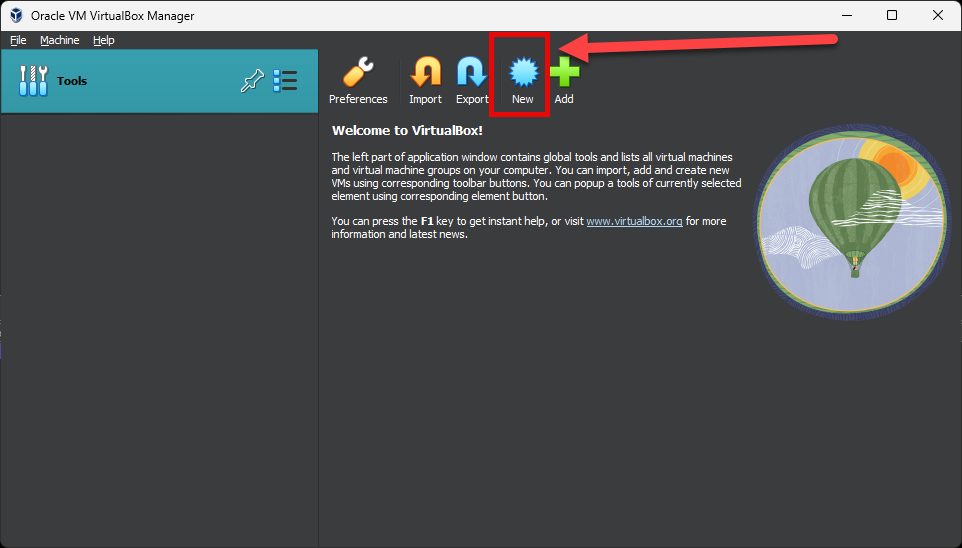
\includegraphics[width=0.7\textwidth]{1.png}
    \caption{Starting the process to create a new virtual machine in VirtualBox.}
\end{figure}

First, we open Oracle VM VirtualBox and click the \textit{New} button to create a new virtual machine.

\section{Configuring the Virtual Machine}
\begin{figure}[H]
    \centering
    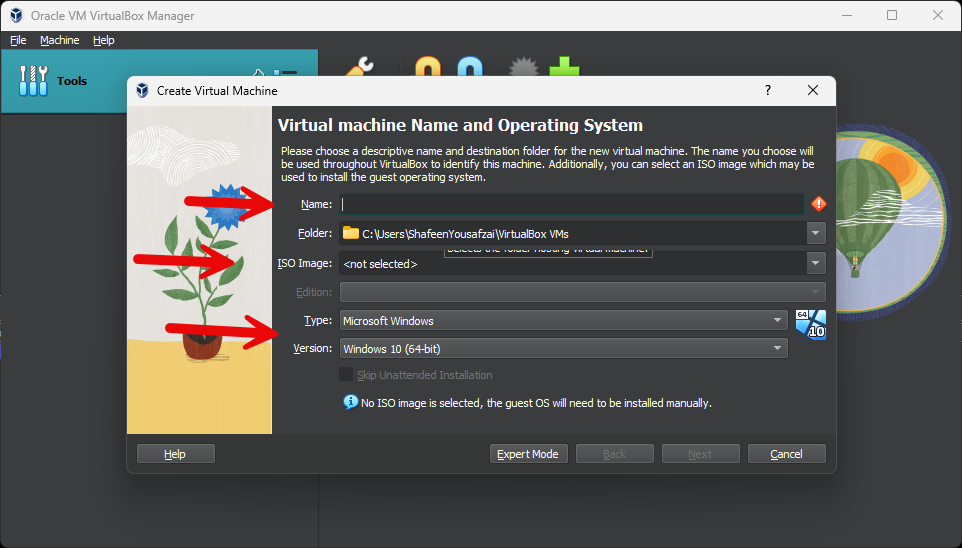
\includegraphics[width=0.7\textwidth]{2.png}
    \caption{Initial configuration window for the new virtual machine.}
\end{figure}

Next, we proceed to the initial setup window for the virtual machine, where we input the machine's name, the location where it will be stored, and the type of operating system that will be installed.

\begin{figure}[H]
    \centering
    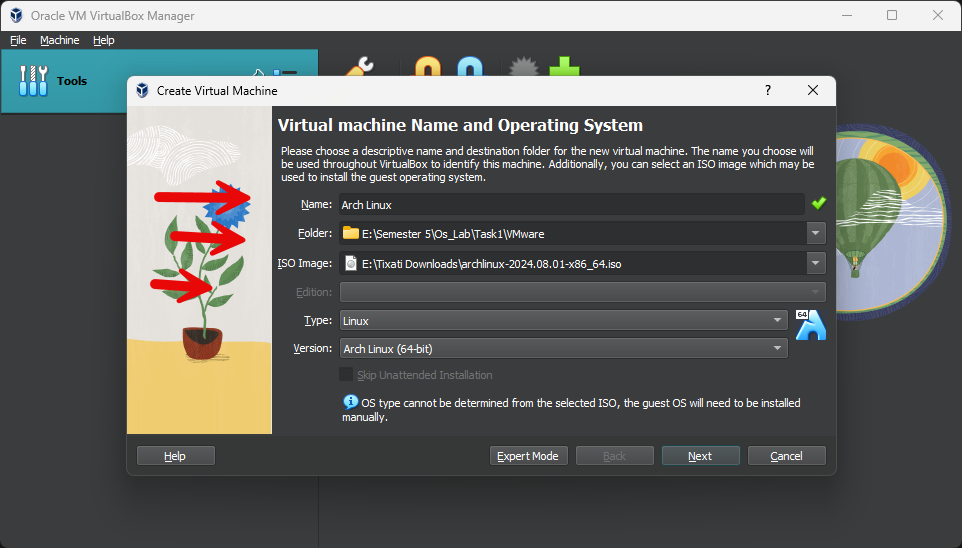
\includegraphics[width=0.7\textwidth]{3.png}
    \caption{Filling in the details for the Arch Linux virtual machine.}
\end{figure}

We fill in the following details:
\begin{itemize}
    \item Name: \textbf{Arch Linux}
    \item Folder: \textit{Path to the virtual machine folder}
    \item ISO Image: \textit{Path to the Arch Linux ISO file}
    \item Type: \textbf{Linux}
    \item Version: \textbf{Arch Linux (64-bit)}
\end{itemize}

\section{Hardware Configuration}
\begin{figure}[H]
    \centering
    
\includegraphics[width=0.7\textwidth]{4.png}
    \caption{Configuring the hardware for the virtual machine.}
\end{figure}

We then configure the virtual machine's hardware as follows:
\begin{itemize}
    \item Base Memory: \textbf{12075 MB (12 GB)}
    \item Processors: \textbf{8 CPUs}
    \item EFI: \textbf{Not enabled}
\end{itemize}

\section{Virtual Hard Disk Setup}
\begin{figure}[H]
    \centering
    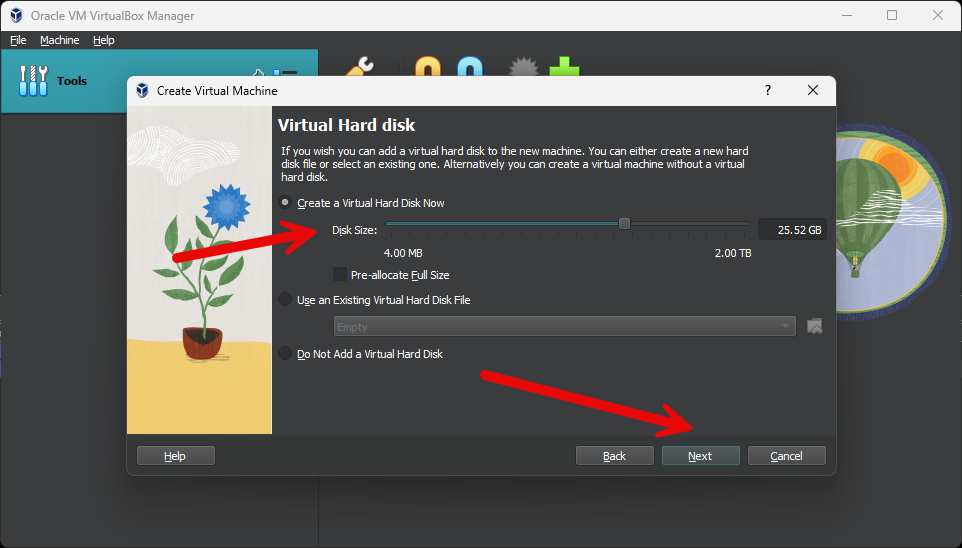
\includegraphics[width=0.7\textwidth]{5.png}
    \caption{Setting up the virtual hard disk.}
\end{figure}

Next, we configure the virtual hard disk with a size of \textbf{25.52 GB} and opt to create a new virtual hard disk.

\section{Summary and Finalization}
\begin{figure}[H]
    \centering
    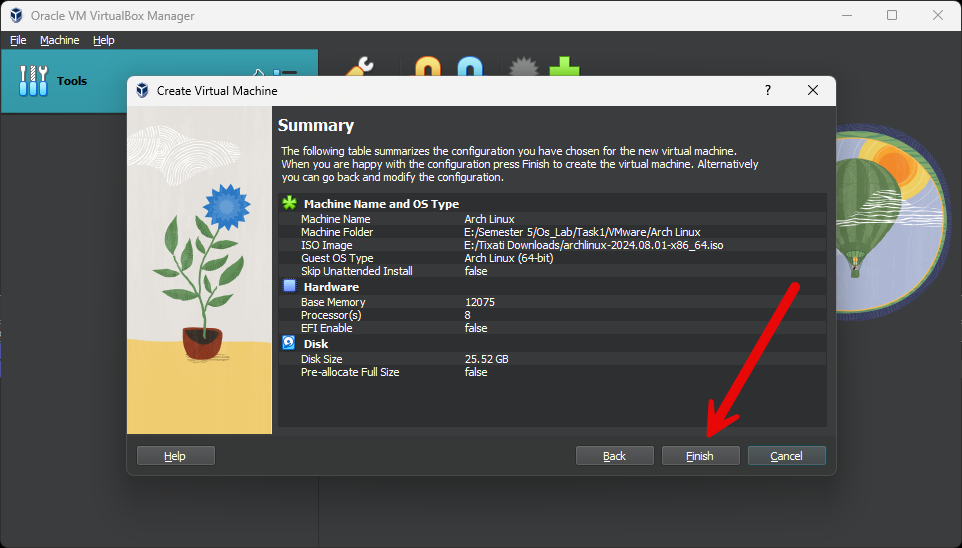
\includegraphics[width=0.7\textwidth]{6.png}
    \caption{Summary of the virtual machine settings.}
\end{figure}

After configuring the hardware and disk, we review the settings and click \textit{Finish} to complete the creation of the virtual machine.

\section{Starting the Virtual Machine}
\begin{figure}[H]
    \centering
    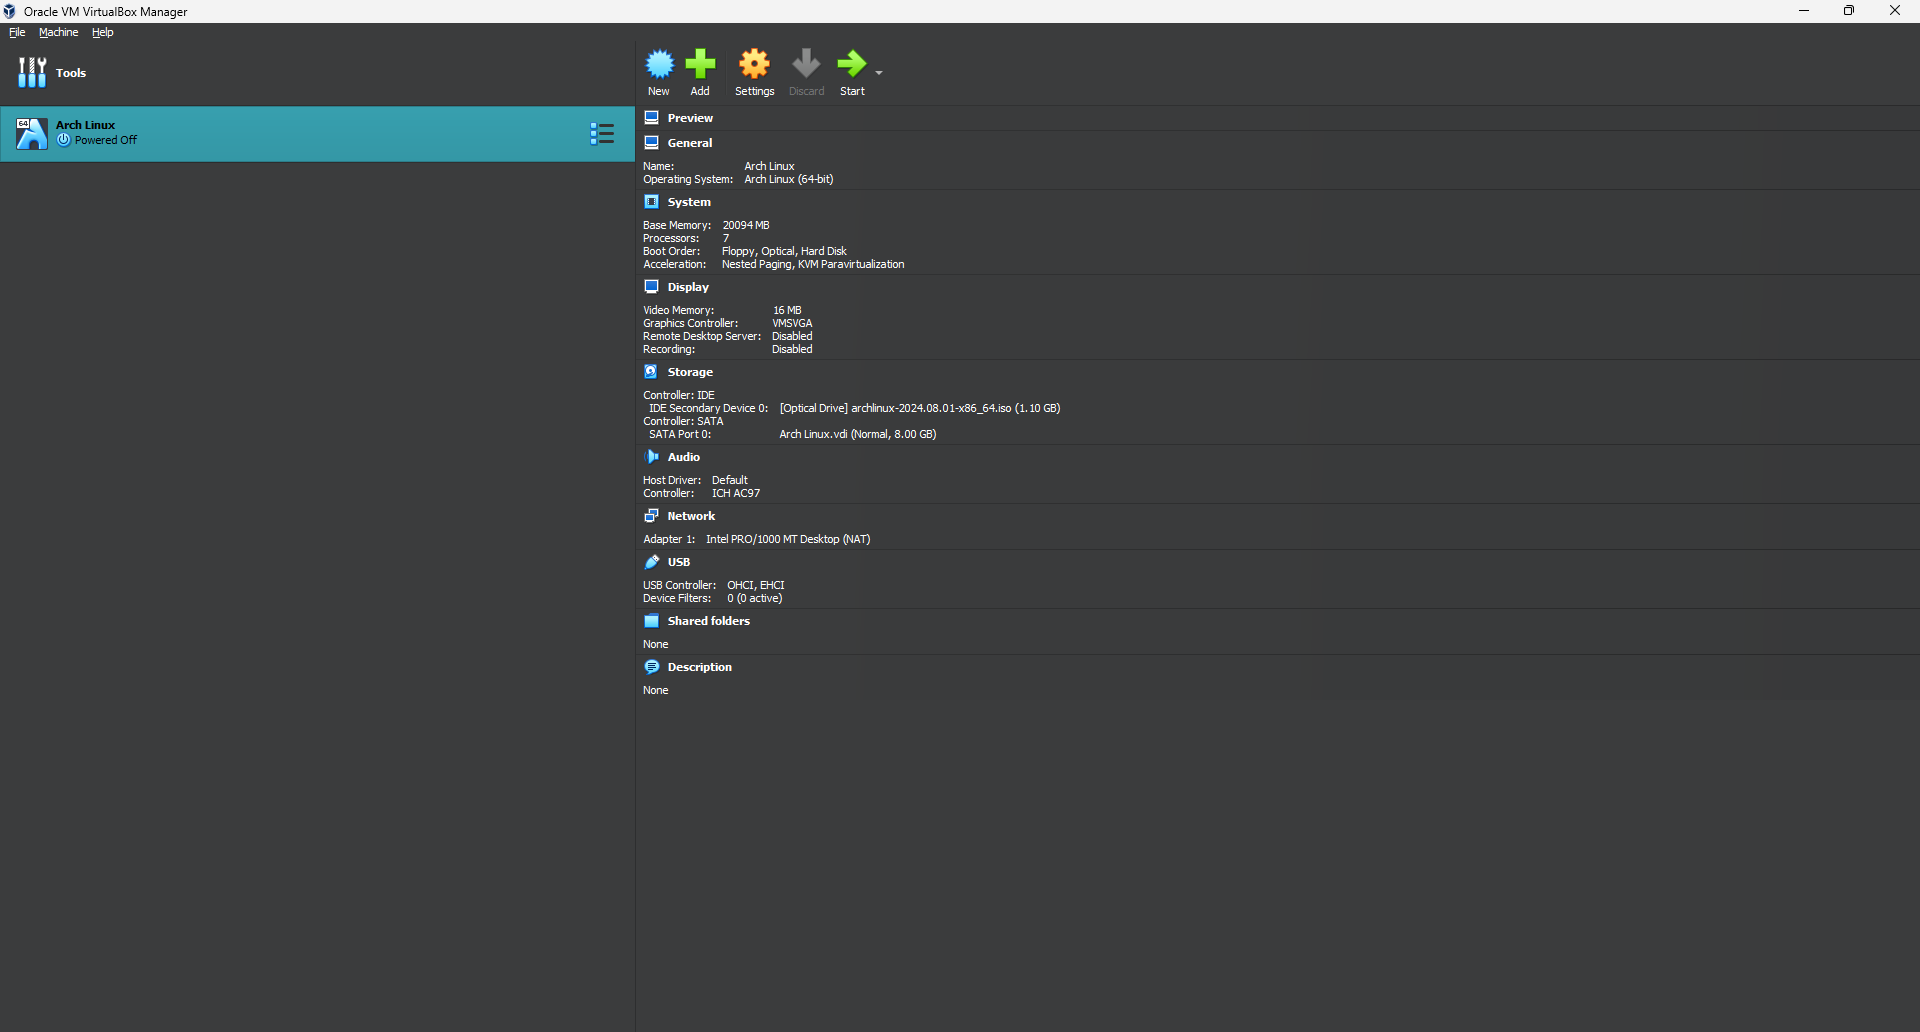
\includegraphics[width=0.7\textwidth]{7.png}
    \caption{VirtualBox Manager showing the newly created Arch Linux virtual machine.}
\end{figure}

With the virtual machine created, it is now listed in the VirtualBox Manager, but it is currently powered off.

\section{Installing Arch Linux}
\begin{figure}[H]
    \centering
    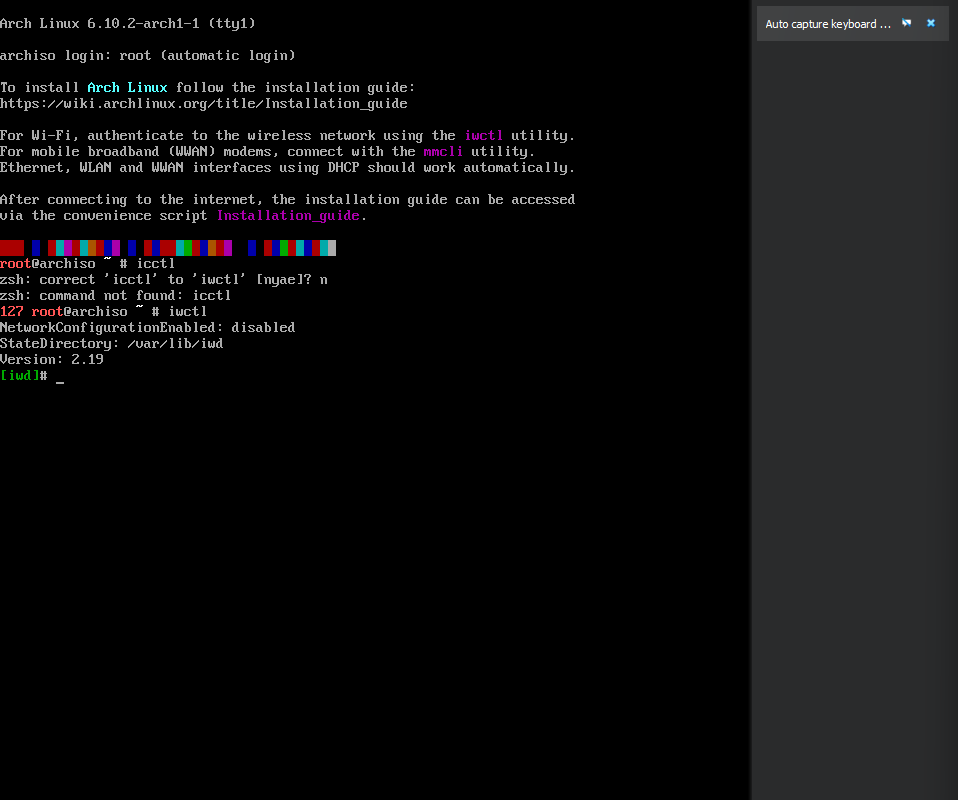
\includegraphics[width=0.7\textwidth]{8.png}
    \caption{Arch Linux command line interface.}
\end{figure}

We start the virtual machine and are greeted with the Arch Linux command line. Here, we enter various setup commands to configure the network and begin the installation.

\begin{figure}[H]
    \centering
    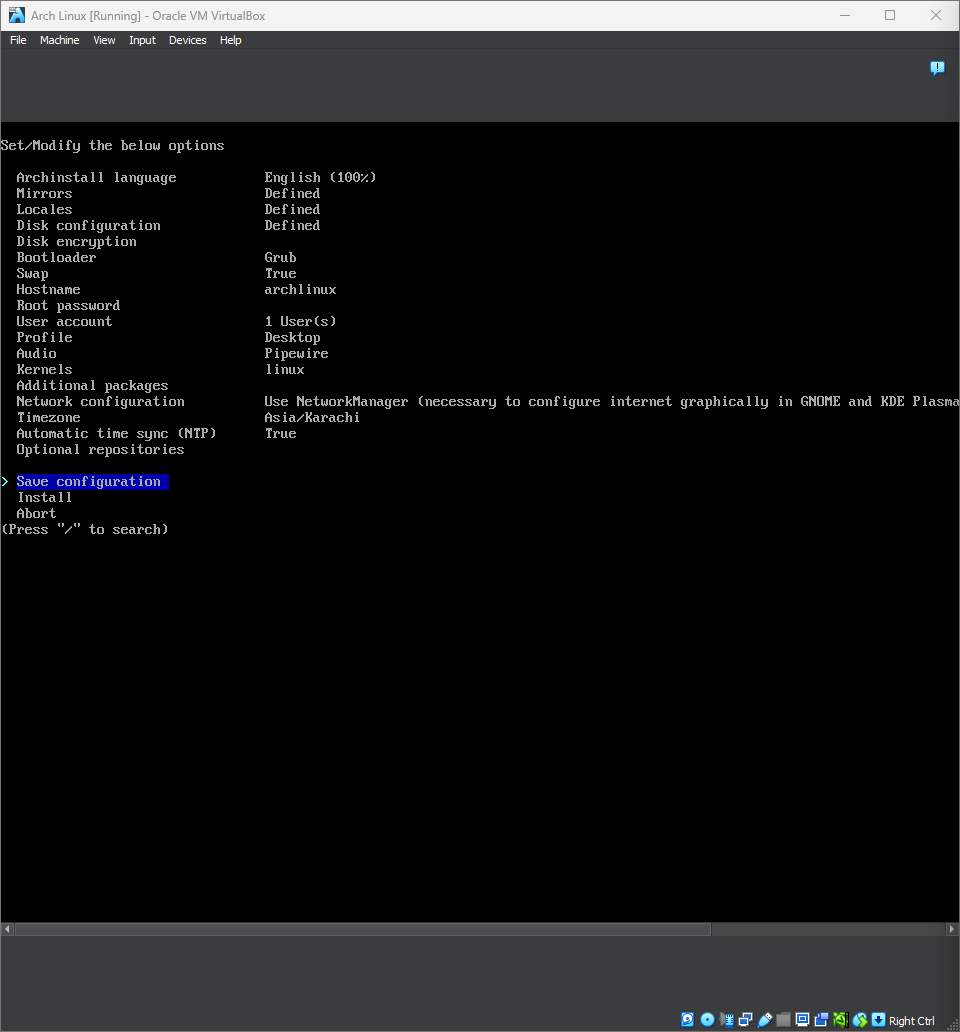
\includegraphics[width=0.7\textwidth]{9.png}
    \caption{Arch Linux installation setup.}
\end{figure}

We navigate through the Arch Linux installation menu, configuring necessary options such as language, mirrors, and disk configuration.

\section{Booting into Arch Linux}
\begin{figure}[H]
    \centering
    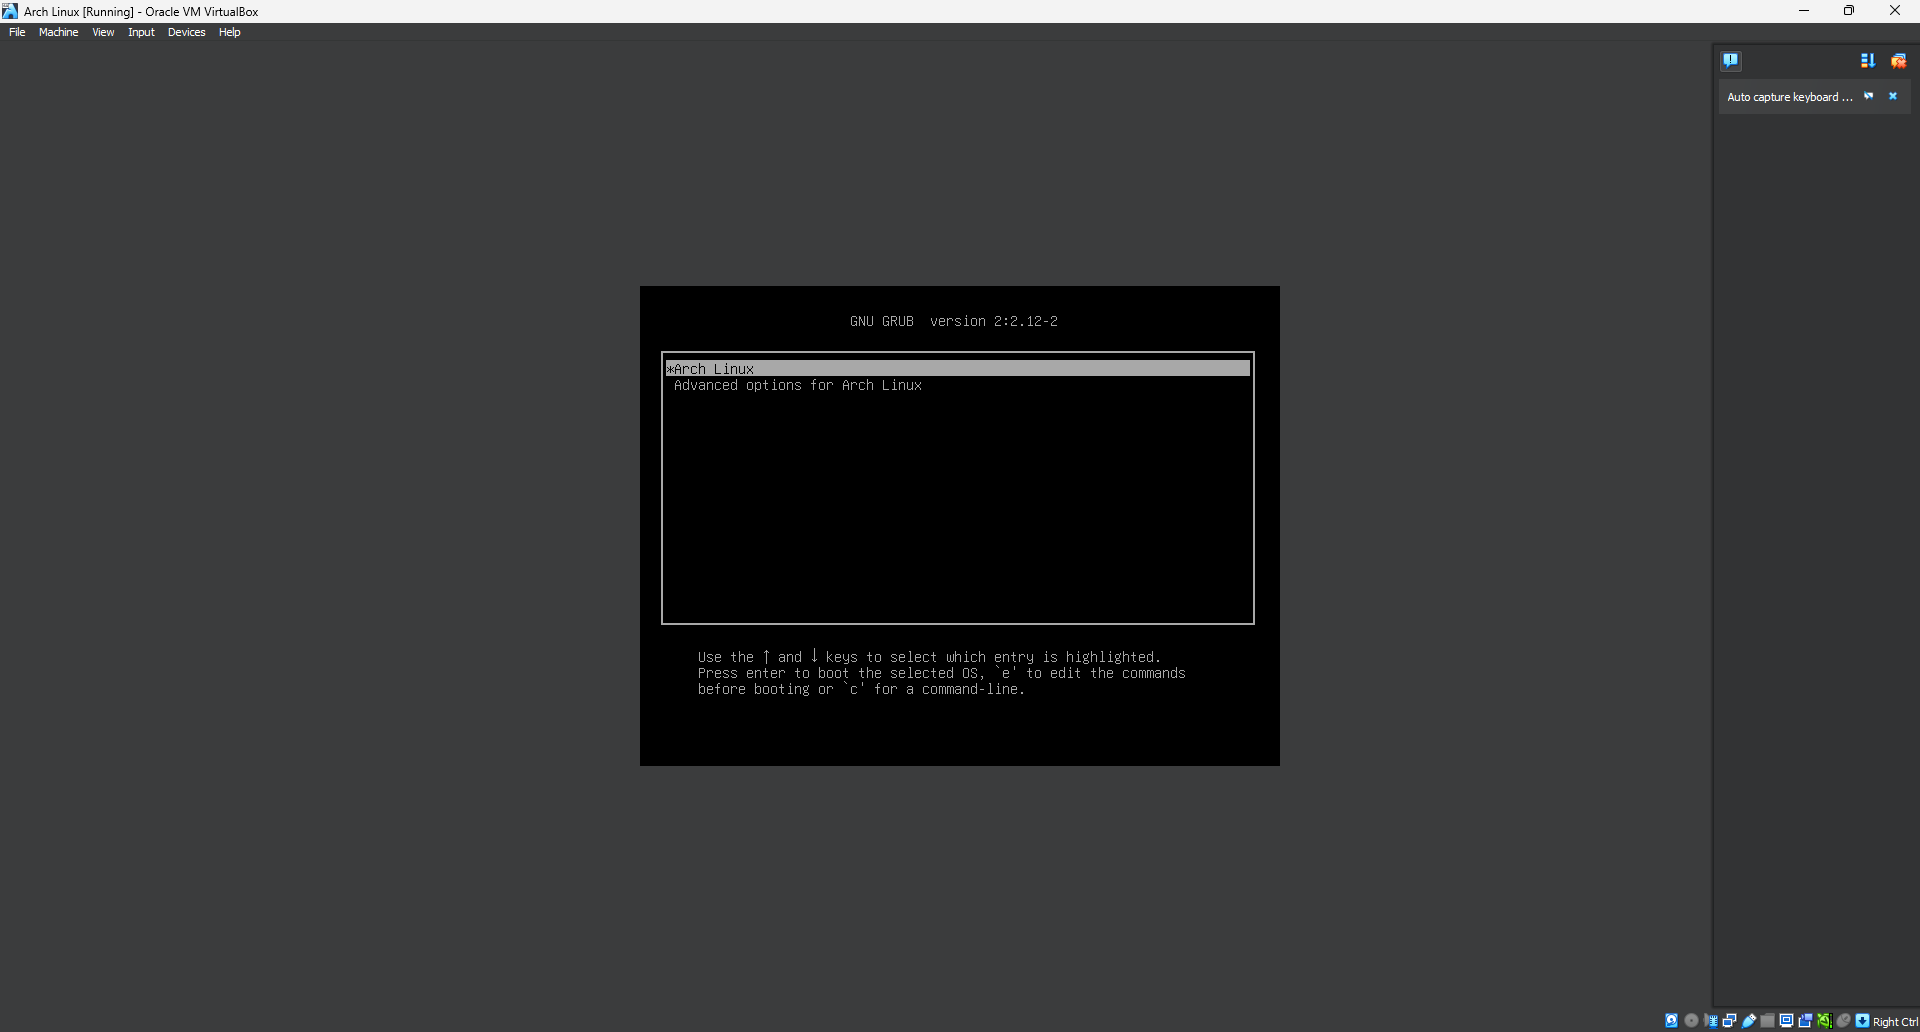
\includegraphics[width=0.7\textwidth]{10.png}
    \caption{GRUB bootloader for Arch Linux.}
\end{figure}

Finally, the GRUB bootloader appears, indicating that Arch Linux is successfully installed and ready to be booted.

\section{Initial Setup After Installation}
\begin{figure}[H]
    \centering
    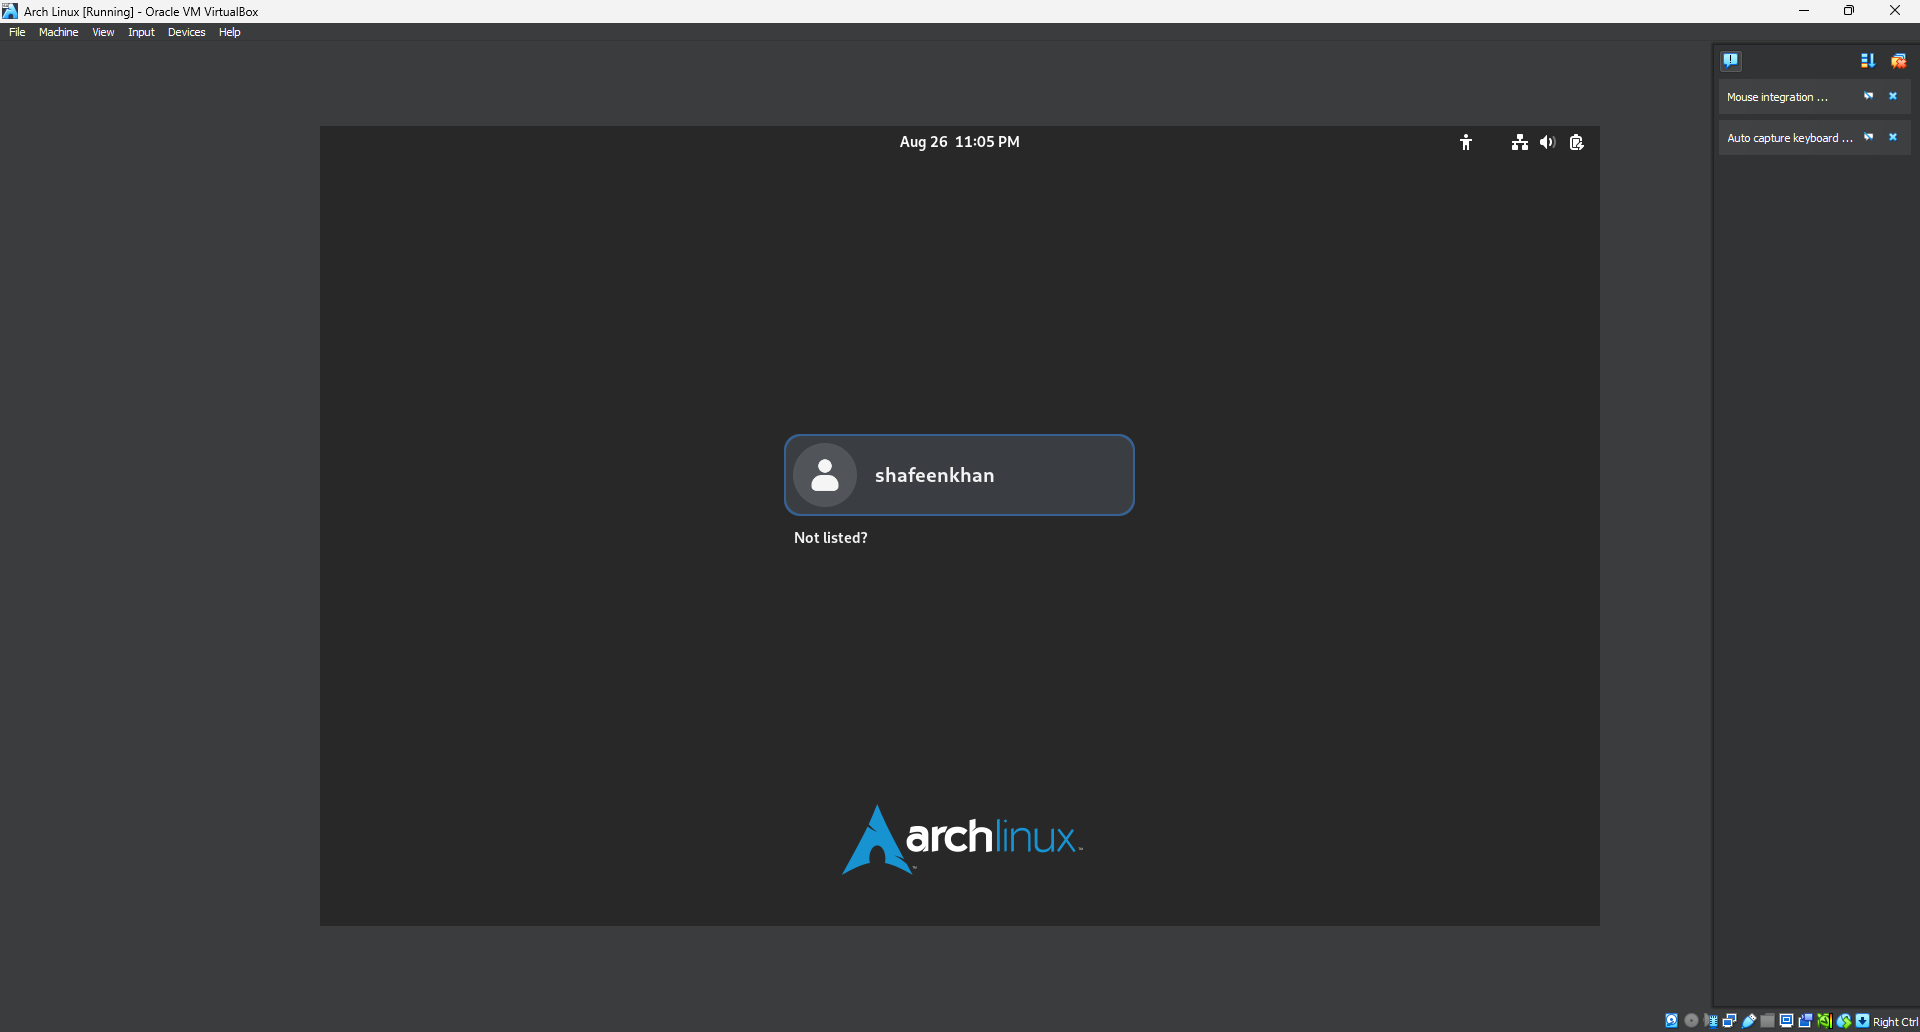
\includegraphics[width=0.7\textwidth]{11.png}
    \caption{Arch Linux login screen.}
\end{figure}

We are now presented with the login screen of Arch Linux, showing that the installation was successful and the system is operational.

\begin{figure}[H]
    \centering
    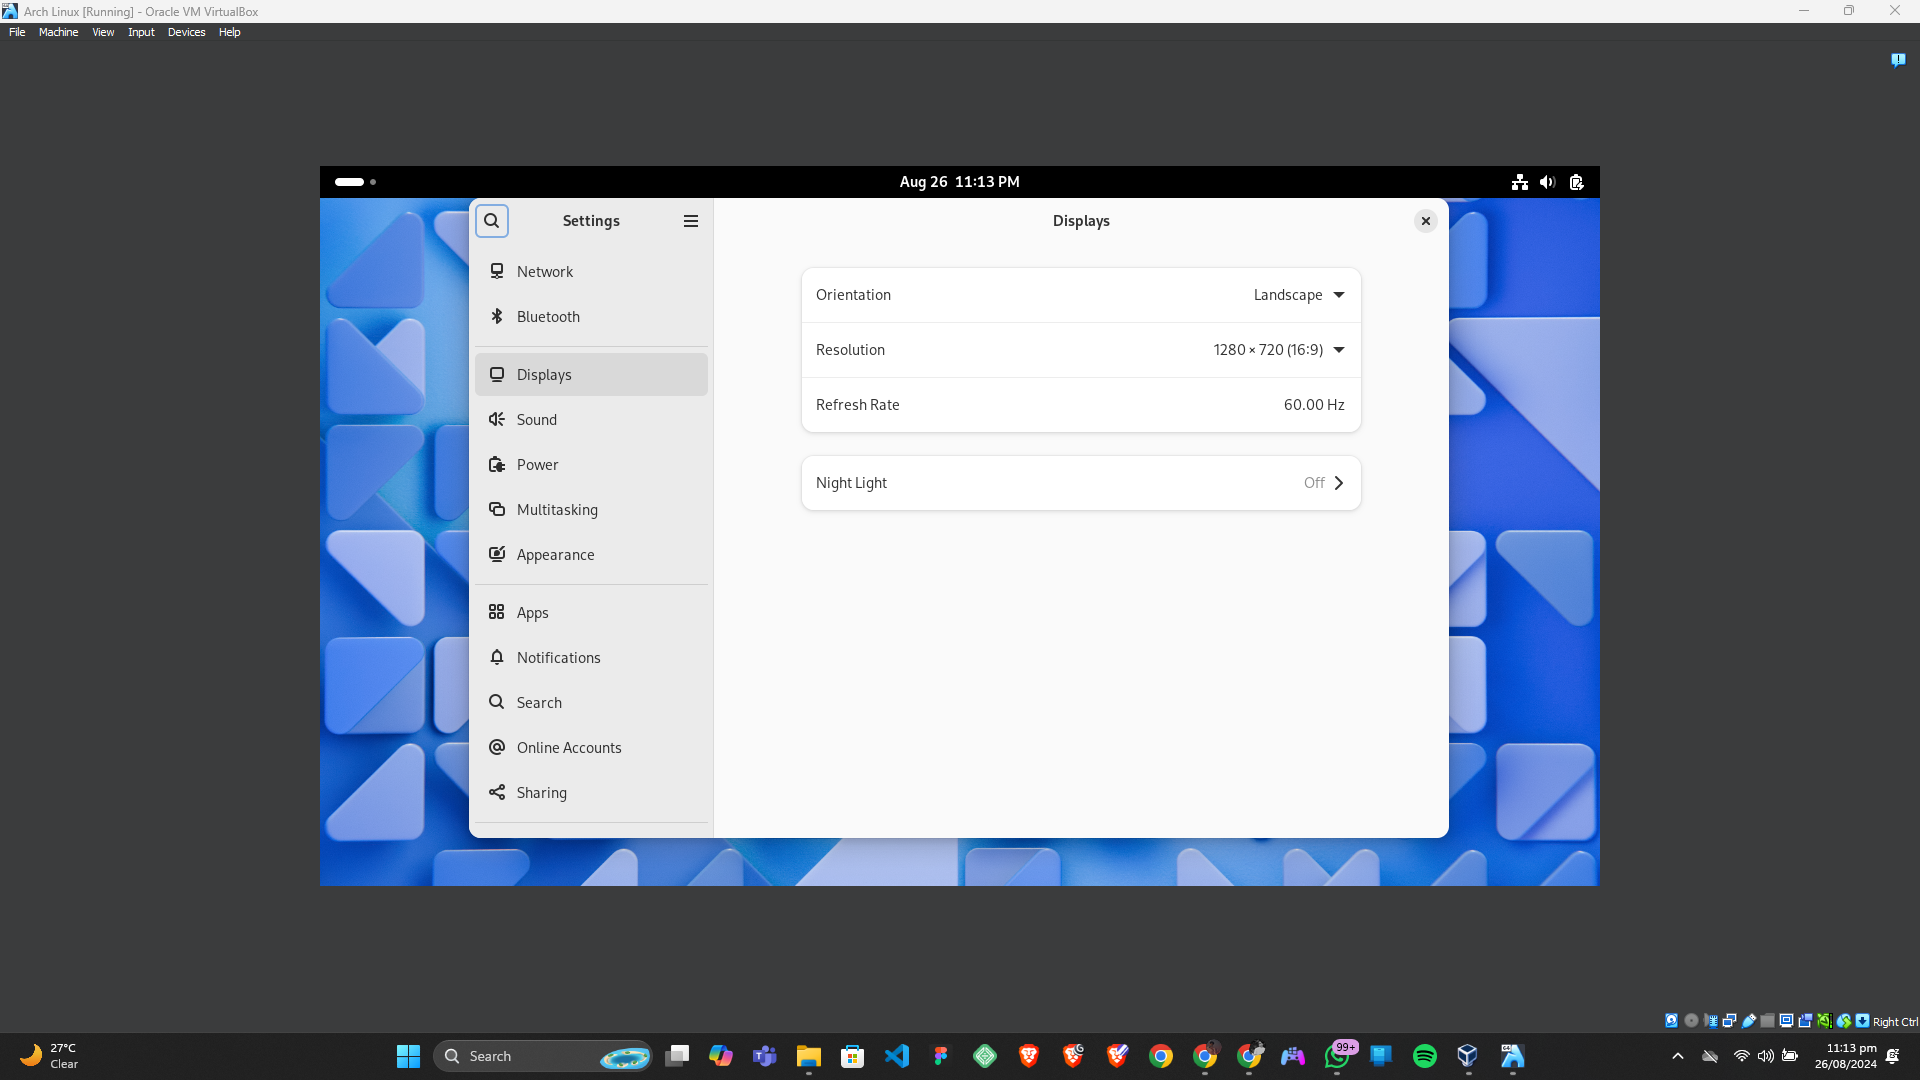
\includegraphics[width=0.7\textwidth]{12.png}
    \caption{Configuring display settings in Arch Linux.}
\end{figure}

After logging in, we proceed to configure the display settings, adjusting the resolution, orientation, and other display parameters.

\section{Conclusion}
The steps outlined in this document successfully demonstrate the process of setting up and installing Arch Linux in Oracle VM VirtualBox. We configured the virtual machine's hardware, created a virtual hard disk, and completed the installation of Arch Linux. The system was successfully booted, and initial setup tasks were performed.

\end{document}
